\documentclass{standalone}
\usepackage{tikz}
\usetikzlibrary{patterns, positioning}


\begin{document}
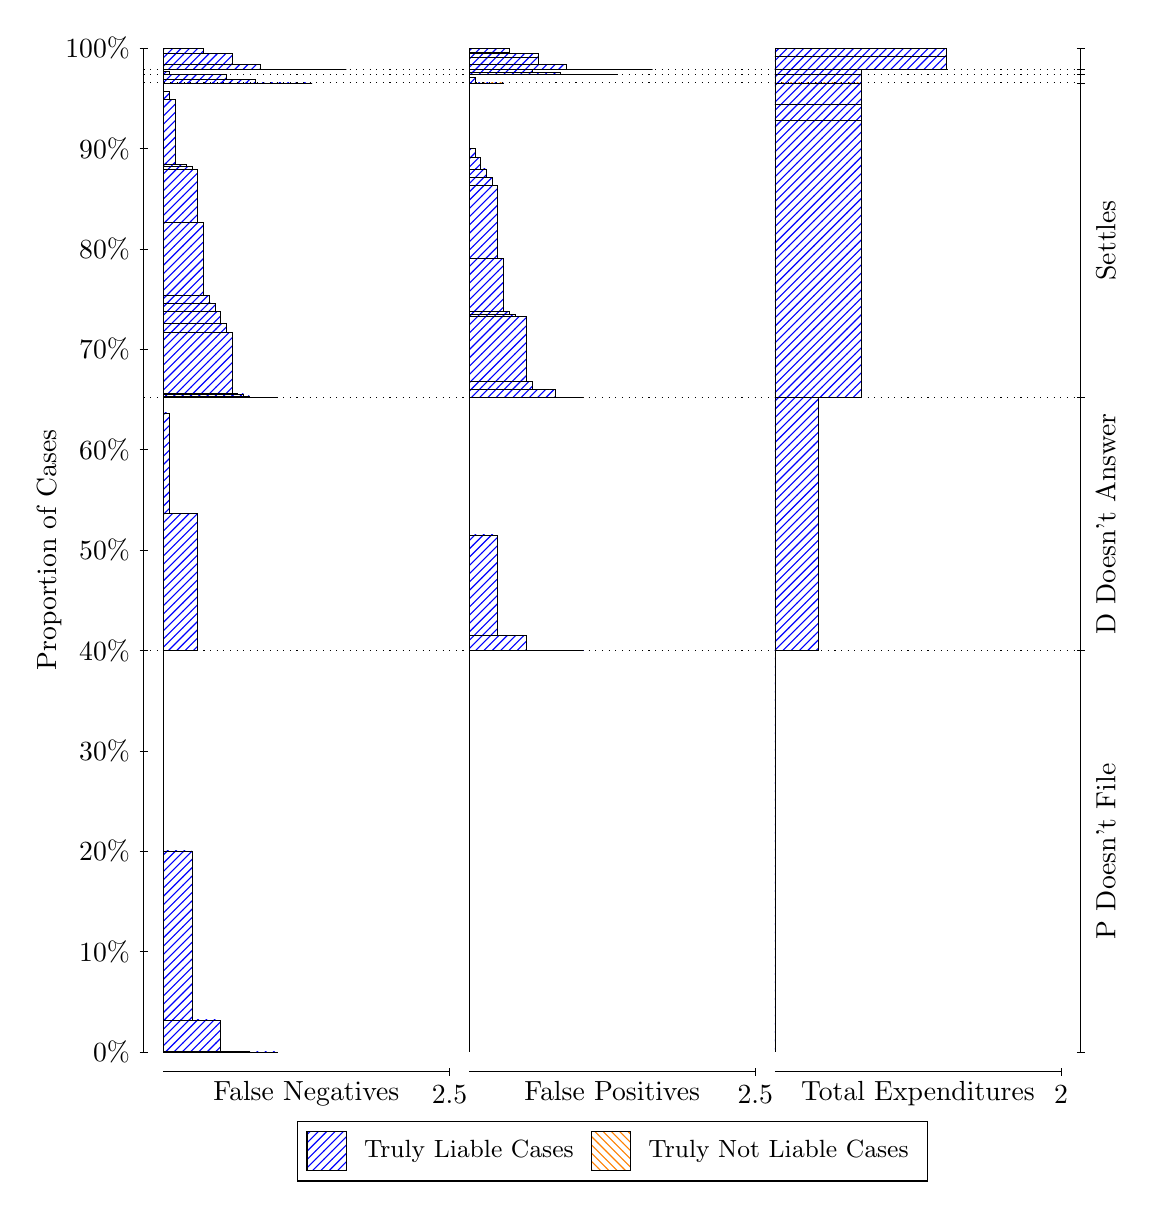
\begin{tikzpicture}
\draw[black, very thin] (1.5,1.75) -- (1.5,14.5);
\node[rotate=90, text=black, anchor=center] at (0.3, 8.125) {Proportion of Cases};
\draw[black, very thin] (1.45,1.75) -- (1.55,1.75);
\node[text=black, anchor=east] at (1.45, 1.75) {0\%};
\draw[black, very thin] (1.45,3.025) -- (1.55,3.025);
\node[text=black, anchor=east] at (1.45, 3.025) {10\%};
\draw[black, very thin] (1.45,4.3) -- (1.55,4.3);
\node[text=black, anchor=east] at (1.45, 4.3) {20\%};
\draw[black, very thin] (1.45,5.575) -- (1.55,5.575);
\node[text=black, anchor=east] at (1.45, 5.575) {30\%};
\draw[black, very thin] (1.45,6.85) -- (1.55,6.85);
\node[text=black, anchor=east] at (1.45, 6.85) {40\%};
\draw[black, very thin] (1.45,8.125) -- (1.55,8.125);
\node[text=black, anchor=east] at (1.45, 8.125) {50\%};
\draw[black, very thin] (1.45,9.4) -- (1.55,9.4);
\node[text=black, anchor=east] at (1.45, 9.4) {60\%};
\draw[black, very thin] (1.45,10.675) -- (1.55,10.675);
\node[text=black, anchor=east] at (1.45, 10.675) {70\%};
\draw[black, very thin] (1.45,11.95) -- (1.55,11.95);
\node[text=black, anchor=east] at (1.45, 11.95) {80\%};
\draw[black, very thin] (1.45,13.225) -- (1.55,13.225);
\node[text=black, anchor=east] at (1.45, 13.225) {90\%};
\draw[black, very thin] (1.45,14.5) -- (1.55,14.5);
\node[text=black, anchor=east] at (1.45, 14.5) {100\%};

\draw[black, very thin] (13.4,1.75) -- (13.4,14.5);
\draw[black, very thin] (13.35,1.75) -- (13.45,1.75);
\node[anchor=west] at (13.35, 1.75) {};
\draw[black, very thin] (13.35,6.8489) -- (13.45,6.8489);
\node[anchor=west] at (13.35, 6.8489) {};
\draw[black, very thin] (13.35,10.06) -- (13.45,10.06);
\node[anchor=west] at (13.35, 10.06) {};
\draw[black, very thin] (13.35,14.057) -- (13.45,14.057);
\node[anchor=west] at (13.35, 14.057) {};
\draw[black, very thin] (13.35,14.164) -- (13.45,14.164);
\node[anchor=west] at (13.35, 14.164) {};
\draw[black, very thin] (13.35,14.227) -- (13.45,14.227);
\node[anchor=west] at (13.35, 14.227) {};
\draw[black, very thin] (13.35,14.5) -- (13.45,14.5);
\node[anchor=west] at (13.35, 14.5) {};

\draw[black, very thin, pattern color=blue, pattern=north east lines] (1.75,1.75) rectangle (3.2033,1.75);
\draw[black, very thin, pattern color=blue, pattern=north east lines] (1.75,1.75) rectangle (2.84,1.7534);
\draw[black, very thin, pattern color=blue, pattern=north east lines] (1.75,1.7534) rectangle (2.4767,2.158);
\draw[black, very thin, pattern color=blue, pattern=north east lines] (1.75,2.158) rectangle (2.1133,4.3029);
\draw[black, very thin, pattern color=orange, pattern=north west lines] (1.75,4.3029) rectangle (1.75,4.3029);
\draw[black, very thin, pattern color=blue, pattern=north east lines] (1.75,4.3029) rectangle (1.75,6.8489);
\draw[black, very thin, pattern color=blue, pattern=north east lines] (1.75,6.8489) rectangle (2.186,8.5931);
\draw[black, very thin, pattern color=blue, pattern=north east lines] (1.75,8.5931) rectangle (1.8227,9.8662);
\draw[black, very thin, pattern color=orange, pattern=north west lines] (1.75,9.8662) rectangle (1.75,9.8662);
\draw[black, very thin, pattern color=blue, pattern=north east lines] (1.75,9.8662) rectangle (1.75,10.06);
\draw[black, very thin, pattern color=blue, pattern=north east lines] (1.75,10.06) rectangle (3.2033,10.06);
\draw[black, very thin, pattern color=blue, pattern=north east lines] (1.75,10.06) rectangle (3.058,10.06);
\draw[black, very thin, pattern color=blue, pattern=north east lines] (1.75,10.06) rectangle (2.9127,10.06);
\draw[black, very thin, pattern color=blue, pattern=north east lines] (1.75,10.06) rectangle (2.84,10.081);
\draw[black, very thin, pattern color=blue, pattern=north east lines] (1.75,10.081) rectangle (2.7673,10.107);
\draw[black, very thin, pattern color=blue, pattern=north east lines] (1.75,10.107) rectangle (2.6947,10.112);
\draw[black, very thin, pattern color=blue, pattern=north east lines] (1.75,10.112) rectangle (2.622,10.889);
\draw[black, very thin, pattern color=blue, pattern=north east lines] (1.75,10.889) rectangle (2.5493,11.007);
\draw[black, very thin, pattern color=blue, pattern=north east lines] (1.75,11.007) rectangle (2.4767,11.153);
\draw[black, very thin, pattern color=blue, pattern=north east lines] (1.75,11.153) rectangle (2.404,11.262);
\draw[black, very thin, pattern color=blue, pattern=north east lines] (1.75,11.262) rectangle (2.3313,11.361);
\draw[black, very thin, pattern color=blue, pattern=north east lines] (1.75,11.361) rectangle (2.2587,12.289);
\draw[black, very thin, pattern color=blue, pattern=north east lines] (1.75,12.289) rectangle (2.186,12.961);
\draw[black, very thin, pattern color=blue, pattern=north east lines] (1.75,12.961) rectangle (2.1133,12.996);
\draw[black, very thin, pattern color=blue, pattern=north east lines] (1.75,12.996) rectangle (2.0407,13.023);
\draw[black, very thin, pattern color=blue, pattern=north east lines] (1.75,13.023) rectangle (1.968,13.028);
\draw[black, very thin, pattern color=blue, pattern=north east lines] (1.75,13.028) rectangle (1.8953,13.851);
\draw[black, very thin, pattern color=blue, pattern=north east lines] (1.75,13.851) rectangle (1.8227,13.953);
\draw[black, very thin, pattern color=orange, pattern=north west lines] (1.75,13.953) rectangle (1.75,13.953);
\draw[black, very thin, pattern color=blue, pattern=north east lines] (1.75,13.953) rectangle (1.75,14.057);
\draw[black, very thin, pattern color=blue, pattern=north east lines] (1.75,14.057) rectangle (3.6393,14.057);
\draw[black, very thin, pattern color=blue, pattern=north east lines] (1.75,14.057) rectangle (3.276,14.057);
\draw[black, very thin, pattern color=blue, pattern=north east lines] (1.75,14.057) rectangle (2.9127,14.097);
\draw[black, very thin, pattern color=blue, pattern=north east lines] (1.75,14.097) rectangle (2.5493,14.163);
\draw[black, very thin, pattern color=blue, pattern=north east lines] (1.75,14.163) rectangle (2.186,14.164);
\draw[black, very thin, pattern color=orange, pattern=north west lines] (1.75,14.164) rectangle (1.75,14.164);
\draw[black, very thin, pattern color=blue, pattern=north east lines] (1.75,14.164) rectangle (2.186,14.165);
\draw[black, very thin, pattern color=blue, pattern=north east lines] (1.75,14.165) rectangle (1.8227,14.203);
\draw[black, very thin, pattern color=orange, pattern=north west lines] (1.75,14.203) rectangle (1.75,14.203);
\draw[black, very thin, pattern color=blue, pattern=north east lines] (1.75,14.203) rectangle (1.75,14.227);
\draw[black, very thin, pattern color=blue, pattern=north east lines] (1.75,14.227) rectangle (4.0753,14.227);
\draw[black, very thin, pattern color=blue, pattern=north east lines] (1.75,14.227) rectangle (3.712,14.227);
\draw[black, very thin, pattern color=blue, pattern=north east lines] (1.75,14.227) rectangle (3.3487,14.231);
\draw[black, very thin, pattern color=blue, pattern=north east lines] (1.75,14.231) rectangle (2.9853,14.294);
\draw[black, very thin, pattern color=blue, pattern=north east lines] (1.75,14.294) rectangle (2.622,14.432);
\draw[black, very thin, pattern color=blue, pattern=north east lines] (1.75,14.432) rectangle (2.2587,14.495);
\draw[black, very thin, pattern color=blue, pattern=north east lines] (1.75,14.495) rectangle (1.8953,14.5);
\draw[black, very thin, pattern color=orange, pattern=north west lines] (1.75,14.5) rectangle (1.75,14.5);
\draw[black, very thin, pattern color=blue, pattern=north east lines] (1.75,14.5) rectangle (1.75,14.5);
\draw[black, very thin, pattern color=orange, pattern=north west lines] (5.6333,1.75) rectangle (5.6333,1.75);
\draw[black, very thin, pattern color=blue, pattern=north east lines] (5.6333,1.75) rectangle (5.6333,6.8489);
\draw[black, very thin, pattern color=orange, pattern=north west lines] (5.6333,6.8489) rectangle (7.0867,6.8489);
\draw[black, very thin, pattern color=blue, pattern=north east lines] (5.6333,6.8489) rectangle (7.0867,6.8489);
\draw[black, very thin, pattern color=blue, pattern=north east lines] (5.6333,6.8489) rectangle (6.7233,6.8492);
\draw[black, very thin, pattern color=blue, pattern=north east lines] (5.6333,6.8492) rectangle (6.36,7.0426);
\draw[black, very thin, pattern color=blue, pattern=north east lines] (5.6333,7.0426) rectangle (5.9967,8.3157);
\draw[black, very thin, pattern color=blue, pattern=north east lines] (5.6333,8.3157) rectangle (5.6333,10.06);
\draw[black, very thin, pattern color=orange, pattern=north west lines] (5.6333,10.06) rectangle (7.0867,10.06);
\draw[black, very thin, pattern color=blue, pattern=north east lines] (5.6333,10.06) rectangle (7.0867,10.06);
\draw[black, very thin, pattern color=orange, pattern=north west lines] (5.6333,10.06) rectangle (6.9413,10.06);
\draw[black, very thin, pattern color=blue, pattern=north east lines] (5.6333,10.06) rectangle (6.9413,10.06);
\draw[black, very thin, pattern color=orange, pattern=north west lines] (5.6333,10.06) rectangle (6.796,10.06);
\draw[black, very thin, pattern color=blue, pattern=north east lines] (5.6333,10.06) rectangle (6.796,10.06);
\draw[black, very thin, pattern color=blue, pattern=north east lines] (5.6333,10.06) rectangle (6.7233,10.163);
\draw[black, very thin, pattern color=orange, pattern=north west lines] (5.6333,10.163) rectangle (6.6507,10.163);
\draw[black, very thin, pattern color=blue, pattern=north east lines] (5.6333,10.163) rectangle (6.6507,10.163);
\draw[black, very thin, pattern color=blue, pattern=north east lines] (5.6333,10.163) rectangle (6.578,10.163);
\draw[black, very thin, pattern color=orange, pattern=north west lines] (5.6333,10.163) rectangle (6.5053,10.163);
\draw[black, very thin, pattern color=blue, pattern=north east lines] (5.6333,10.163) rectangle (6.5053,10.163);
\draw[black, very thin, pattern color=blue, pattern=north east lines] (5.6333,10.163) rectangle (6.4327,10.266);
\draw[black, very thin, pattern color=blue, pattern=north east lines] (5.6333,10.266) rectangle (6.36,11.089);
\draw[black, very thin, pattern color=blue, pattern=north east lines] (5.6333,11.089) rectangle (6.2873,11.094);
\draw[black, very thin, pattern color=blue, pattern=north east lines] (5.6333,11.094) rectangle (6.2147,11.121);
\draw[black, very thin, pattern color=blue, pattern=north east lines] (5.6333,11.121) rectangle (6.142,11.156);
\draw[black, very thin, pattern color=blue, pattern=north east lines] (5.6333,11.156) rectangle (6.0693,11.828);
\draw[black, very thin, pattern color=blue, pattern=north east lines] (5.6333,11.828) rectangle (5.9967,12.756);
\draw[black, very thin, pattern color=blue, pattern=north east lines] (5.6333,12.756) rectangle (5.924,12.855);
\draw[black, very thin, pattern color=blue, pattern=north east lines] (5.6333,12.855) rectangle (5.8513,12.964);
\draw[black, very thin, pattern color=blue, pattern=north east lines] (5.6333,12.964) rectangle (5.7787,13.11);
\draw[black, very thin, pattern color=blue, pattern=north east lines] (5.6333,13.11) rectangle (5.706,13.227);
\draw[black, very thin, pattern color=blue, pattern=north east lines] (5.6333,13.227) rectangle (5.6333,14.057);
\draw[black, very thin, pattern color=orange, pattern=north west lines] (5.6333,14.057) rectangle (6.0693,14.057);
\draw[black, very thin, pattern color=blue, pattern=north east lines] (5.6333,14.057) rectangle (6.0693,14.058);
\draw[black, very thin, pattern color=blue, pattern=north east lines] (5.6333,14.058) rectangle (5.706,14.124);
\draw[black, very thin, pattern color=blue, pattern=north east lines] (5.6333,14.124) rectangle (5.6333,14.164);
\draw[black, very thin, pattern color=orange, pattern=north west lines] (5.6333,14.164) rectangle (7.5227,14.164);
\draw[black, very thin, pattern color=blue, pattern=north east lines] (5.6333,14.164) rectangle (7.5227,14.164);
\draw[black, very thin, pattern color=blue, pattern=north east lines] (5.6333,14.164) rectangle (7.1593,14.164);
\draw[black, very thin, pattern color=blue, pattern=north east lines] (5.6333,14.164) rectangle (6.796,14.188);
\draw[black, very thin, pattern color=blue, pattern=north east lines] (5.6333,14.188) rectangle (6.4327,14.226);
\draw[black, very thin, pattern color=blue, pattern=north east lines] (5.6333,14.226) rectangle (6.0693,14.227);
\draw[black, very thin, pattern color=orange, pattern=north west lines] (5.6333,14.227) rectangle (7.9587,14.227);
\draw[black, very thin, pattern color=blue, pattern=north east lines] (5.6333,14.227) rectangle (7.9587,14.227);
\draw[black, very thin, pattern color=orange, pattern=north west lines] (5.6333,14.227) rectangle (7.5953,14.227);
\draw[black, very thin, pattern color=blue, pattern=north east lines] (5.6333,14.227) rectangle (7.5953,14.227);
\draw[black, very thin, pattern color=orange, pattern=north west lines] (5.6333,14.227) rectangle (7.232,14.227);
\draw[black, very thin, pattern color=blue, pattern=north east lines] (5.6333,14.227) rectangle (7.232,14.232);
\draw[black, very thin, pattern color=blue, pattern=north east lines] (5.6333,14.232) rectangle (6.8687,14.294);
\draw[black, very thin, pattern color=orange, pattern=north west lines] (5.6333,14.294) rectangle (6.8687,14.294);
\draw[black, very thin, pattern color=blue, pattern=north east lines] (5.6333,14.294) rectangle (6.8687,14.295);
\draw[black, very thin, pattern color=blue, pattern=north east lines] (5.6333,14.295) rectangle (6.5053,14.384);
\draw[black, very thin, pattern color=orange, pattern=north west lines] (5.6333,14.384) rectangle (6.5053,14.384);
\draw[black, very thin, pattern color=blue, pattern=north east lines] (5.6333,14.384) rectangle (6.5053,14.433);
\draw[black, very thin, pattern color=blue, pattern=north east lines] (5.6333,14.433) rectangle (6.142,14.446);
\draw[black, very thin, pattern color=blue, pattern=north east lines] (5.6333,14.446) rectangle (6.142,14.496);
\draw[black, very thin, pattern color=blue, pattern=north east lines] (5.6333,14.496) rectangle (5.7787,14.496);
\draw[black, very thin, pattern color=blue, pattern=north east lines] (5.6333,14.496) rectangle (5.7787,14.5);
\draw[black, very thin, pattern color=blue, pattern=north east lines] (5.6333,14.5) rectangle (5.6333,14.5);
\draw[black, very thin, pattern color=orange, pattern=north west lines] (9.5167,1.75) rectangle (9.5167,1.75);
\draw[black, very thin, pattern color=blue, pattern=north east lines] (9.5167,1.75) rectangle (9.5167,6.8489);
\draw[black, very thin, pattern color=orange, pattern=north west lines] (9.5167,6.8489) rectangle (10.062,6.8489);
\draw[black, very thin, pattern color=blue, pattern=north east lines] (9.5167,6.8489) rectangle (10.062,10.06);
\draw[black, very thin, pattern color=orange, pattern=north west lines] (9.5167,10.06) rectangle (10.607,10.06);
\draw[black, very thin, pattern color=blue, pattern=north east lines] (9.5167,10.06) rectangle (10.607,13.583);
\draw[black, very thin, pattern color=orange, pattern=north west lines] (9.5167,13.583) rectangle (10.607,13.583);
\draw[black, very thin, pattern color=blue, pattern=north east lines] (9.5167,13.583) rectangle (10.607,13.786);
\draw[black, very thin, pattern color=orange, pattern=north west lines] (9.5167,13.786) rectangle (10.607,13.786);
\draw[black, very thin, pattern color=blue, pattern=north east lines] (9.5167,13.786) rectangle (10.607,14.057);
\draw[black, very thin, pattern color=orange, pattern=north west lines] (9.5167,14.057) rectangle (10.607,14.057);
\draw[black, very thin, pattern color=blue, pattern=north east lines] (9.5167,14.057) rectangle (10.607,14.164);
\draw[black, very thin, pattern color=orange, pattern=north west lines] (9.5167,14.164) rectangle (10.607,14.164);
\draw[black, very thin, pattern color=blue, pattern=north east lines] (9.5167,14.164) rectangle (10.607,14.227);
\draw[black, very thin, pattern color=orange, pattern=north west lines] (9.5167,14.227) rectangle (11.697,14.227);
\draw[black, very thin, pattern color=blue, pattern=north east lines] (9.5167,14.227) rectangle (11.697,14.397);
\draw[black, very thin, pattern color=orange, pattern=north west lines] (9.5167,14.397) rectangle (11.697,14.397);
\draw[black, very thin, pattern color=blue, pattern=north east lines] (9.5167,14.397) rectangle (11.697,14.5);
\draw[black, dotted] (1.5,6.8489) -- (13.4,6.8489);
\draw[black, dotted] (1.5,10.06) -- (13.4,10.06);
\draw[black, dotted] (1.5,14.057) -- (13.4,14.057);
\draw[black, dotted] (1.5,14.164) -- (13.4,14.164);
\draw[black, dotted] (1.5,14.227) -- (13.4,14.227);
\draw[black, very thin] (1.75,1.5) -- (5.3833,1.5);
\node[text=black, anchor=north] at (3.5667, 1.5) {False Negatives};
\draw[black, very thin] (5.3833,1.45) -- (5.3833,1.55);
\node[text=black, anchor=north] at (5.3833, 1.45) {2.5};

\draw[black, very thin] (5.6333,1.5) -- (9.2667,1.5);
\node[text=black, anchor=north] at (7.45, 1.5) {False Positives};
\draw[black, very thin] (9.2667,1.45) -- (9.2667,1.55);
\node[text=black, anchor=north] at (9.2667, 1.45) {2.5};

\draw[black, very thin] (9.5167,1.5) -- (13.15,1.5);
\node[text=black, anchor=north] at (11.333, 1.5) {Total Expenditures};
\draw[black, very thin] (13.15,1.45) -- (13.15,1.55);
\node[text=black, anchor=north] at (13.15, 1.45) {2};

\node[text=black, centered, rotate=90] at (13.72, 4.2994) {P Doesn't File};
\node[text=black, centered, rotate=90] at (13.72, 8.4544) {D Doesn't Answer};
\node[text=black, centered, rotate=90] at (13.72, 12.058) {Settles};




\draw (7.449999999999999,1.5) node[draw=none] (baseCoordinate) {};
\begin{scope}[align=center]
        \matrix[scale=0.5, draw=black, below=0.5cm of baseCoordinate, nodes={draw}, column sep=0.1cm]{
            \node[rectangle, draw, minimum width=0.5cm, minimum height=0.5cm, pattern color=blue, pattern=north east lines] {}; &
            \node[draw=none, font=\small, text=black] (B) {Truly Liable Cases}; &
            \node[rectangle, draw, minimum width=0.5cm, minimum height=0.5cm, pattern color=orange, pattern=north west lines] {}; &
            \node[draw=none, font=\small, text=black] (B) {Truly Not Liable Cases}; \\
            };
\end{scope}

\end{tikzpicture}
\end{document}